% 11/23/2015
%%%%%%%%%%%%%%%%%%%%%%%%%%%%%%%%%%%%%%%%%%%%%%%%%%%%%%%%%%%%%%%%%%%%%%%%%%%%
% AGUJournalTemplate.tex: this template file is for articles formatted with LaTeX
%
% This file includes commands and instructions
% given in the order necessary to produce a final output that will
% satisfy AGU requirements. 
%
% You may copy this file and give it your
% article name, and enter your text.
%
%%%%%%%%%%%%%%%%%%%%%%%%%%%%%%%%%%%%%%%%%%%%%%%%%%%%%%%%%%%%%%%%%%%%%%%%%%%%
% PLEASE DO NOT USE YOUR OWN MACROS
% DO NOT USE \newcommand, \renewcommand, or \def, etc.
%
% FOR FIGURES, DO NOT USE \psfrag or \subfigure.
% DO NOT USE \psfrag or \subfigure commands.
%%%%%%%%%%%%%%%%%%%%%%%%%%%%%%%%%%%%%%%%%%%%%%%%%%%%%%%%%%%%%%%%%%%%%%%%%%%%
%
% All questions should be e-mailed to latex@agu.org.
%
%%%%%%%%%%%%%%%%%%%%%%%%%%%%%%%%%%%%%%%%%%%%%%%%%%%%%%%%%%%%%%%%%%%%%%%%%%%%
%
% Step 1: Set the \documentclass
%
% There are two options for article format:
%
% 1) PLEASE USE THE DRAFT OPTION TO SUBMIT YOUR PAPERS.
% The draft option produces double spaced output.
% 
% 2) numberline will give you line numbers.

%% To submit your paper:
%\documentclass[draft,linenumbers]{agujournal}
%\draftfalse

%% For final version.
\documentclass{agujournal}
\usepackage{url}
%\newcommand*{\gi}[1]{\overline{\overline{#1}}}
\newcommand*{\gi}[1]{\widehat{#1}}
\usepackage{graphicx}%for gnuplot epslatex
% Now, type in the journal name: \journalname{<Journal Name>}

% ie, \journalname{Journal of Geophysical Research}
%% Choose from this list of Journals:
%
% JGR-Atmospheres
% JGR-Biogeosciences
% JGR-Earth Surface
% JGR-Oceans
% JGR-Planets
% JGR-Solid Earth
% JGR-Space Physics
% Global Biochemical Cycles
% Geophysical Research Letters
% Paleoceanography
% Radio Science
% Reviews of Geophysics
% Tectonics
% Space Weather
% Water Resource Research
% Geochemistry, Geophysics, Geosystems
% Journal of Advances in Modeling Earth Systems (JAMES)
% Earth's Future
% Earth and Space Science
%
%

\journalname{Journal of Advances in Modeling Earth Systems (JAMES)}


\begin{document}

%% ------------------------------------------------------------------------ %%
%  Title
% 
% (A title should be specific, informative, and brief. Use
% abbreviations only if they are defined in the abstract. Titles that
% start with general keywords then specific terms are optimized in
% searches)
%
%% ------------------------------------------------------------------------ %%

% Example: \title{This is a test title}

\title{A detailed total energy and physics-dynamics coupling analysis of the Community Atmosphere Model (CAM)}

%% ------------------------------------------------------------------------ %%
%
%  AUTHORS AND AFFILIATIONS
%
%% ------------------------------------------------------------------------ %%

% Authors are individuals who have significantly contributed to the
% research and preparation of the article. Group authors are allowed, if
% each author in the group is separately identified in an appendix.)

% List authors by first name or initial followed by last name and
% separated by commas. Use \affil{} to number affiliations, and
% \thanks{} for author notes.  
% Additional author notes should be indicated with \thanks{} (for
% example, for current addresses). 

% Example: \authors{A. B. Author\affil{1}\thanks{Current address, Antartica}, B. C. Author\affil{2,3}, and D. E.
% Author\affil{3,4}\thanks{Also funded by Monsanto.}}

\authors{P.H. Lauritzen\affil{1}\thanks{1850 Table Mesa Drive, Boulder, Colorado, USA}, and D.L. Williamson \affil{1}}

 \affiliation{1}{National Center for Atmospheric Research, Boulder, Colorado, USA}
% \affiliation{2}{School of Marine and Atmospheric Sciences, Stony Brook University, State University of New York, Stony Brook, New York}
% \affiliation{3}{Sandia National Laboratories, Albuquerque, New Mexico, USA}
% \affiliation{4}{Department of Land, Air and Water Resources, University of California, Davis, California, USA}
% \affiliation{5}{Ecole Polytechnique, UMR 8539, Laboratoire de M\'et\'eorologie Dynamique/IPSL, Palaiseau, France}
% \affiliation{6}{Rosenstiel School of Marine and Atmospheric Science, University of Miami, Miami, Florida, USA}

% \affiliation{3}{Third Affiliation}
% \affiliation{4}{Fourth Affiliation}

%(repeat as many times as is necessary)

%% Corresponding Author:
% Corresponding author mailing address and e-mail address:

% (include name and email addresses of the corresponding author.  More
% than one corresponding author is allowed in this LaTeX file and for
% publication; but only one corresponding author is allowed in our
% editorial system.)  

% Example: \correspondingauthor{First and Last Name}{email@address.edu}

\correspondingauthor{Peter Hjort Lauritzen}{pel@ucar.edu}

%% Keypoints, final entry on title page.

% Example: 
% \begin{keypoints}
% \item	List up to three key points (at least one is required)
% \item	Key Points summarize the main points and conclusions of the article
% \item	Each must be 100 characters or less with no special characters or punctuation 
% \end{keypoints}

%  List up to three key points (at least one is required)
%  Key Points summarize the main points and conclusions of the article
%  Each must be 100 characters or less with no special characters or punctuation 

\begin{keypoints}
\item ...
%\item The CESM2.0 release of the spectral-element dynamical core (CAM-SE) is documented
%\item Model has comprehensive treatment of condensates and energy
%\item The CAM-SE model has been sped-up significantly compared to its predecessor CAM-HOMME
\end{keypoints}

%% ------------------------------------------------------------------------ %%
%
%  ABSTRACT
%
% A good abstract will begin with a short description of the problem
% being addressed, briefly describe the new data or analyses, then
% briefly states the main conclusion(s) and how they are supported and
% uncertainties. 
%% ------------------------------------------------------------------------ %%

%% \begin{abstract} starts the second page 

\begin{abstract}

\end{abstract}


%% ------------------------------------------------------------------------ %%
%
%  TEXT
%
%% ------------------------------------------------------------------------ %%

%%% Suggested section heads:
%\section{Introduction}
% 
% The main text should start with an introduction. Except for short
% manuscripts (such as comments and replies), the text should be divided
% into sections, each with its own heading. 

% Headings should be sentence fragments and do not begin with a
% lowercase letter or number. Examples of good headings are:

% \section{Materials and Methods}
% Here is text on Materials and Methods.
%
% \subsection{A descriptive heading about methods}
% More about Methods.
% 
% \section{Data} (Or section title might be a descriptive heading about data)
% 
% \section{Results} (Or section title might be a descriptive heading about the
% results)
% 
% \section{Conclusions}


\section{Introduction}
In coupled climate modeling with prognostic atmosphere, ocean, land, land-ice, and sea-ice components, it is important to conserve total energy (TE) to a high degree to avoid spurious long term trends in the simulated Earth system. Conservation of TE in this context refers to having a closed TE budget. For example, the TE change in a column in the atmosphere is exactly balanced by the net sources/sinks given by the fluxes through the column. The fluxes into the atmospheric component from the surface models must be balanced by the fluxes in the respective surface components and so on. Henceforth we will focus only on the atmospheric component which, in a numerical model, is split into a resolved-scale component (the dynamical core) and a sub-grid-scale component (parameterizations or, in modeling jargon, physics). 

The atmospheric equations of motion conserve TE but the discretizations used in climate and weather models are usually not inherently TE conservative. Exact conservation is probably not necessary but conservation to within $~$0.01  $W/m^2$ has been considered sufficient to avoid spurious trends in century long simulations \citep{B2000S,WOHTTV2015JAMES}. Spurious sources and sinks of TE can be introduced by the dynamical core, physics, physics-dynamics coupling as well as discrepancies between the TE of the continuous and discrete equations of motion and for the physics. Hence the study of TE conservation in comprehensive models of the atmosphere quickly becomes a quite complex and detailed matter. In addition there can easily be compensating errors in the system as a whole.

Here we focus on versions of the Community Atmosphere Model (CAM) that use the spectral-element \citep[SE, ][]{LetAl2018JAMES} and finite-volume \citep[FV, ][]{L2004MWR} dynamical cores. These dynamical cores couple with physics in a time-split manner, i.e. physics receives a state updated by dynamics \citep[see ][ for a discussion of time-split versus process split physics-dynamics coupling in the context of CAM]{W2002MWR}.

In its pure time-split form the physics tendencies are added to the state previously produced by the dynamical core and the resulting state provides the initial state for the subsequent dynamical core calculation. We refer to this as state-updating. Alternatively, when the dynamical core adopts a shorter time step than the physics, say $nsplit$ sub-steps, then (1/$nsplit$)th of the physics-calculated tendency is added to the state before each dynamics sub-step. We refer to this modification of time-splitting as {\em{dribbling}}. CAM-FV uses the state-update approach while CAM-SE has options to use state-update, {\em{dribbling}} or a combination of the two (i.e. mass-variables use state-updating and others use {\em{dribbling}}). The dribbling variants can lead to spurious sources or sinks of TE referred to as physics-dynamics coupling errors.

The dynamical core usually has implicit or explicit filters to control spurious noise near the grid scale which will lead to energy dissipation \citep{T2008JCP,JW2010LNCSE}. Similarly models often have sponge layers to control the solution near the top of the model that may be a sink of TE. There are examples of numerical discretizations of the adiabatic frictionless equations motion that are designed so that TE is conserved in the absence of time-truncation and filtering errors, e.g., mimetic spectral-element discretizations such as the one used in the horizontal in CAM-SE \citep{T2011LNCSEb}. These provide consistency between the discrete momentum and thermodynamic equations leading to global conservation associated with the conversion of potential to kinetic energy. In spectral transform models it is customary to add the energy change due to explicit diffusion on momentum back as heating (referred to as frictional heating), so that the diffusion of momentum does not affect the TE budget \citep[see, e.g., p.71 in ][]{CAM5}. This is also done in CAM-SE \citep{LetAl2018JAMES}. 

It is the purpose of this paper to provide a provide a detailed global TE analysis of CAM. We assess TE dissipation due to various steps in the model algorithms. The paper is outlined as follows. In the Methods section the continuous TE formulas are given and a detailed description of spurious TE sources/sinks that can occur in a model as a whole, and the associated diagnostics used to perform the detailed TE analysis are defined. In the Results section the model is run in various configuration to assess the effects on TE sources/sinks. This includes various physics-dynamics coupling experiments. In this context a rather detailed discussion of mass budget closure is given.


%For example, the discrete TE consistent with the dynamical core may differ from the one used in physics or,  even worse, the TE that the continuous equations of motion conserve is different between the dynamical core and physics.\\

\section{Method}
\subsection{Defining total energy (TE)}\label{sec:defE}
In the following it is assumed that the model top and bottom are coordinate surfaces and that there is no flux of mass through the model top and bottom. In a dry atmosphere the TE equation integrated over the entire sphere is given by
\begin{equation}
\frac{d}{dt}\int_{z=z_s}^{z=z_{top}}\iint_{\Omega} E_v \rho^{(d)}\, dA\, dz=\int_{z=z_s}^{z=z_{top}}\iint_{\Omega} F_{net}\, \rho^{(d)} dA\, dz,
\end{equation}
\citep[e.g., ][]{K1974MWR} where $F_{net}$ is net fluxes calculated by the parameterizations (e.g., heating and momentum forcing), $d/dt$ the total/material derivative, $z_s$ is the height of the surface, $\Omega$ the sphere, $\rho^{(d)}$ the density of dry air and $E_v$ is the TE. $E_v$ can be split into kinetic energy $K=\frac{1}{2}\vec{v}^2$ ($\mathbf{v}$ is the wind vector), internal energy $c_v^{(d)}T$, where $c_v^{(d)}$ is the heat capacity of dry air at constant volume, and potential energy $\Phi=gz$
\begin{equation}
E_v=K+c_v^{(d)}T+\Phi.
\end{equation}
If the vertical integral is performed in a mass-based vertical coordinate, e.g., pressure, then the integrated TE equation for a dry atmosphere can be written as
\begin{equation}
\frac{d}{dt}\int_{p=p_s}^{p=p_{top}}\iint_{\Omega} E_p \rho^{(d)}\, dA\, dp + \frac{d}{dt}\iint_{\Omega}\Phi_sp_s dA =\int_{p=p_s}^{p=p_{top}}\iint_{\Omega} F_{net}\, \rho dA\, dp,
\end{equation}
\citep[e.g., ][]{K1974MWR} where
\begin{equation}
E_p=K+c_p^{(d)}T.
\end{equation}
In a moist atmosphere, however, there are several definitions of TE used in the literature related to what heat capacity is used for water vapor and whether or not condensates are accounted for in the energy equation. To explain the details of that we focus on the energy equation for CAM-SE.

CAM-SE is formulated using a terrain-following hybrid-sigma vertical coordinate $\eta$ but the coordinate levels are defined in terms of dry air mass ($M^{(d)}$) instead of total air mass; $\eta^{(d)}$ \citep[see ][ for details]{LetAl2018JAMES}. In such a coordinate system it is convenient to define the tracer state in terms of a dry mixing ratio instead of moist mixing ratio
\begin{equation}
m^{(\ell)}\equiv \frac{\rho^{(\ell)}}{\rho^{(d)}}, \text{ where }\ell=`wv`,`cl`,`ci`,`rn`,`sw`,\label{eq:mx}
\end{equation}
where $\rho^{(d)}$ is the mass of dry air per unit volume of moist air and $\rho^{(\ell)}$ is the mass of the water substance of type $\ell$ per unit volume of moist air. Moist air refers to air containing dry air (`d`), water vapor (`wv`), cloud liquid (`cl`), cloud ice (`ci`), rain amount(`rn`) and snow amount(`sw`). For notational purposes define the set of all components of air
\begin{equation}
\mathcal{L}_{all}=\left\{ `d`,`wv`,`cl`,`ci`,`rn`,`sw`\right\},
\end{equation}
Define associated heat capacities at constant pressure $c_p^{(\ell)}$. Using the $\eta^{(d)}$ vertical coordinate and dry mixing ratios the TE that the frictionless adiabatic equations of motion in the CAM-SE dynamical core conserves is 
\begin{equation}
\gi{E}_{dyn}=\int_{\eta=0}^{\eta=1} \iint_\mathcal{S} \left( \frac{\partial M^{(d)}}{\partial \eta^{(d)}} \right)\sum_{\ell \in \mathcal{L}_{all}} \left[m^{(\ell)} \left(K+c_p^{(\ell)}T+\Phi_s  \right)\right]  dA d \eta^{(d)},\label{eq:comprehensice_energy}
\end{equation}
where $\Phi_s$ is the surface geopotential and $\gi{(\cdot)}$ refers to the global integral.

In the CAM physical parameterizations a different definition of TE is used. Due to the evolutionary nature of the model development, the parameterizations have not yet been converted to match the SE dynamical core. For the computation of TE condensates are assumed to be zero and the heat capacity of moisture is the same as for dry air. This is equivalent to using a moist mass (dry air plus water vapor) but $c_p$ of dry air:
\begin{equation}
\label{eq:Ephys}
\gi{E}_{phys} =\int_{\eta=0}^{\eta=1} \iint_\mathcal{S} \left( \frac{\partial M^{(d)}}{\partial \eta^{(d)}} \right)\left(1+m^{(wv)}\right)\left[ \left(K+c_p^{(d)}T+\Phi_s\right)\right]dA d \eta^{(d)}.
\end{equation}
We note that earlier versions of CAM using the spectral transform dynamical core used $c_p$ of moist air. 
One can make the adiabatic, frictionless equations of motion in the dynamical core conserve $E^{(physics)}$ by not including condensates in the mass/pressure field as well as energy conversion term in the thermodynamic equation and setting the heat capacity for moisture to $c_p^{(d)}$ \citep{T2011LNCSEb}. We refer to this version of CAM-SE as the {\em{energy consistent}} version.


\subsection{Spurious energy sources and sinks}\label{subsec:spuriousE}
In a weather/climate model TE conservation errors can appear in many places throughout the algorithm. Below is a general list of where conservation errors can appear with specific examples from CAM:
\begin{enumerate}
\item {\em{Parameterization errors}}: Individual parameterizations may not have a closed energy budget. CAM parameterizations are required to have a closed energy budget under the assumption that pressure remains constant during the computation of the subgrid-scale parameterization tendencies. In other words, the TE change in the column is exactly balanced by the net sources/sinks given by the fluxes through the column. 
\item {\em{Pressure work}}: That said, if parameterizations update specific humidity then the surface pressure changes (e.g., moisture leaving the column). In that case the pressure changes which, in turn, changes TE. This is referred to as {\em{pressure work}} \citep[section 3.1.8 in ][]{CAM5}.
\item {\em{Continuous TE formula discrepancy}}:  If the continuous equations of motion for the dynamical core conserve a TE different from the one used in the parameterizations then an energy inconsistency is present in the system as a whole. This is the case with the new version of CAM-SE that conserves a TE that is more accurate and comprehensive than the CAM physics package as discussed above. As also noted above, this mismatch arose from the evolutionary nature of the model development and not by deliberate design.
\item {\em{Dynamical core errors}}: Energy conservation errors in the dynamical core, not related to PDC errors, can arise in multiple parts of the algorithms used to solve the equations of motion. For dynamical cores employing implicit filtering \citep[e.g., limiters in flux operators ][]{L2004MWR} and/or possessing inherent damping to control small scales, it is hard to diagnose what their energy dissipation is compared to other errors in the discretization. If explicit filtering is used, e.g., hyperviscosity on momentum, then one can diagnose the energy dissipation from filtering and add a corresponding heating to balance it. There may also be energy loss from viscosity applied to other variables such a temperature or surface pressure which are harder to compensate. Here is a beak-down relevant to CAM-SE using a floating Lagrangian vertical coordinate:
\begin{itemize}
\item Horizontal inviscid dynamics: Energy errors resulting from solving the inviscid, adiabatic equations of motion.
\item Hyperviscosity: Filtering errors.
\item Vertical remapping: The vertical remapping algorithm does not conserve TE.
\item Near round-off negative values
\end{itemize}
\item {\em{Physics-dynamics coupling (PDC)}}: Assume that physics computes a tendency. Usually the tendency is passed to the dynamical core which is responsible for adding the tendencies to the state. PDC energy errors can be split into two types:
\begin{itemize}
\item {\em{`Dribbling' errors (or, equivalently, temporal PDC errors)}}: If the TE increment from the parameterizations does not match the change in TE when the tendencies are added to the state in the dynamical core, then there will be a spurious PDC error. This will not happen with the state-update approach in which the tendencies are added immediate after physics and before the dynamical core advances the solution in time, but it does happen with dribbling. 
\item {\em{Change of vertical grid/coordinate errors}}: If the vertical coordinate in physics and in the dynamical core are different then there can be spurious PDC energy errors even when using the state-update method for adding tendencies to the dynamical core state. For example, many non-hydrostatic dynamical cores \citep[e.g. MPAS, ]{MPASatm} use a terrain-following height coordinate whereas physics uses pressure.
\item {\em{Change of horizontal grid errors:}} If the physics tendencies are computed on a different horizontal grid than the dynamical core then there can be spurious energy errors from mapping tendencies between horizontal grids \citep[e.g., ][]{HetAl2018MWR}. 
\end{itemize}
\end{enumerate}
To avoid TE conservation errors which could accumulate and ultimately lead to a climate drift, it is customary to use an energy fixer to restore TE conservation. Since the spatial distribution of energy errors, in general, is not known, global fixers are used. In CAM a uniform increment is added to the temperature field to compensate for TE loss in the dynamical core, physics-dynamics coupling, TE formula discrepancy and energy change due to pressure work. 

\subsection{Diagnostics}
The discrete global integrals $\gi{(\cdot)}$ are computed consistent with the discrete model grid as outlined in section 2.2. of \citet{LBDL2014JAMES}. The TE tendency is denoted
\begin{equation}
\partial \gi{E}\equiv \frac{d\gi{E}}{dt}.
\end{equation}
By computing the global TE integrals $\gi{E}$ at appropriate places in the model algorithms, we can directly compute $\partial \gi{E}$ due to various processes (such as viscosity, vertical remapping, physics-dynamics coupling, pressure work etc.) by differencing $\gi{E}$ from after and before the algorithm step is taking place. This has been implemented using CAM history infrastructure that internally handles accumulation and averaging. The places in CAM where we compute/capture $\gi{E}$ are named using three letters where the first letter refers to whether the integral is performed in physics (`p') or in the dynamical core (`d'). The trailing to letters refer to the specific location in dynamics or physics. For example, 'BF' refers to `Before energy Fixer' and `AF' to `After energy Fixer'; the associated total energies are denoted $\gi{E}_{pBF}$ and $\gi{E}_{pAF}$, respectively. The TE tendency of the energy fixer is the difference between $\gi{E}_{pBF}$ and $\gi{E}_{pAF}$ divided by the time-step. The pseudo-code in Figure \ref{fig:dAD} defines the acronyms in terms of where in the CAM-SE algorithm the global TE integrals are computed and output. For details on the CAM-SE algorithm please see \citet{LetAl2018JAMES}.

\begin{figure}[h]
% \centering
% when using pdflatex, use pdf file:

\verb+do nt=1,ntotal+\\
\verb+  +\\
\verb+  PARAMETERIZATIONS:+\\
\verb+  +\\
\verb+  +{\color{blue}{output 'pBF'}}\\
\verb+  +Energy fixer\\
\verb+  +{\color{blue}{output 'pBP'}}\\
\verb+  +Physics updates the state and state saved for energy fixer\\
\verb+  +{\color{blue}{output 'pAP'}}\\
\verb+  +Dry mass correction\\
\verb+  +{\color{blue}{output 'pAM'}}\\
\verb+  +\\
\verb+  DYNAMICAL CORE:+\\
\verb+  +\\
\verb+  +{\color{blue}{output 'dED'}}\\
\verb+  do ns=1,nsplit+\\
\verb+    +{\color{blue}{output 'dAF'}}\\
\verb+    Update state with (1/nsplit) of the physics tendencies (ftype=2)+\\
\verb+    if (ns==1) Update state with entire physics tendency (ftype=1)+\\
\verb+    +{\color{blue}{output 'dBD'}}\\
\verb+    do nr=1,rsplit+\\
\verb+       Advance the adiabatic frictionless equations of motion +\\
\verb+       in floating Lagrangian layer.+\\
\verb+       do ns=1,hypervis_subcycle+\\
\verb+          +{\color{blue}{output 'dBH'}}\\
\verb+          Advance hyperviscosity operators.+\\
\verb+          +{\color{blue}{output 'dCH'}}\\
\verb+          Add frictional heating to temperature.+\\
\verb+          +{\color{blue}{output 'dAH'}}\\
\verb+       end do+\\
\verb+    end do+\\
\verb+    +{\color{blue}{output 'dAD'}}\\
\verb+    Vertical remapping from floating Lagrangian levels to Eulerian levels+\\
\verb+    +{\color{blue}{output 'dAR'}}\\
\verb+  end do+\\
\verb+  +{\color{blue}{output 'dBF'}}\\
\verb+end do+
\caption{Pseudo-code for CAM-SE. {\color{red}{more text needed; define all the splits and nested loops}}}
\label{fig:dAD}
\end{figure}


Define the following energy tendencies (corresponding to itemized list in section \ref{subsec:spuriousE}):
\begin{enumerate}
%
\item $\partial \gi{E}^{(param)}$: TE tendency due to parameterizations. In CAM the TE budget for each parameterization is closed (assuming constant pressure) so $\partial \gi{E}^{(param)}$ are balanced by net fluxes in/out of the physics columns. Note that this is the only energy tendency that is not spurious since CAM parameterizations have a closed energy budget. This TE tendency is discretely computed as
\begin{equation}
\partial \gi{E}_{phys}^{({param})}=\frac{\gi{E}_{pAP}-\gi{E}_{pBP}}{\Delta t_{phys}},
\end{equation}
where $\Delta t_{phys}$ is the physics time-step (1800s) and the subscript $phys$ refers to the energy tendency being computed in CAM physics. 
%
\item $\partial \gi{E}^{({pwork})}$: Total spurious energy tendency due to pressure work
\begin{equation}
\partial \gi{E}_{phys}^{({pwork})}=\frac{\gi{E}_{pAM}-\gi{E}_{pAP}}{\Delta t_{phys}}.
\end{equation}
Since CAM-SE is based on a dry-mass vertical coordinate the pressure work takes place implicitly in the dynamical core.

The total forcing from physics (at least in CAM) consists of parameterizations, pressure work and TE fixer, with associated energy tendency
\begin{equation}
\partial \gi{E}_{phys}^{({efix})}=\frac{\gi{E}_{pBP}-\gi{E}_{pBF}}{\Delta t_{phys}}.
\end{equation}
When all the TE budget terms have been defined it will be discussed further exactly what comprises $\partial \gi{E}_{phys}^{({efix})}$.

For notational convenience we refer to the associated energy tendency from all of physics as
\begin{equation}
\partial \gi{E}_{phys}^{({phys})}\equiv \partial \gi{E}_{phys}^{({param})}+\partial \gi{E}_{phys}^{({pwork})}+\partial \gi{E}_{phys}^{({efix})}=\frac{\gi{E}_{pAM}-\gi{E}_{pBF}}{\Delta t_{phys}}.
\end{equation}
\item $\partial \gi{E}^{({discr})}$: If the physics uses a TE definition different from the TE that the continuous equations of motion in the dynamical core conserve (in the absence of dicretization errors), then there is a TE discrepancy tendency. This complicates the energy analysis as one can not compare TE computed in physics $\gi{E}_{phys}$ directly with TE computed in the dynamical core $\gi{E}_{dyn}$. This makes errors associated with this discrepancy tricky to assess. That said, the TE tendencies computed using the dynamical core TE formula $\partial \gi{E}_{dyn}$ are well defined (self consistent) and similarly for TE tendencies computed using the `physics formula' for TE: $\partial \gi{E}_{phys}$.


\item The TE tendency from the dynamical core is split into several terms:
\begin{itemize} 
\item Horizontal adiabatic dynamics (dynamics excluding physics forcing tendency)
\begin{equation}
\partial \gi{E}_{dyn}^{({2D})}=\frac{\gi{E}_{dAD}-\gi{E}_{dBD}}{\Delta t_{dyn}},
\end{equation}
where $\Delta t_{dyn}=\frac{\Delta t_{phys}}{nsplit\times rsplit}$.

In CAM-SE the viscosity is explicit so one can compute the TE tendency due to hyperviscosity
\begin{equation}
\partial \gi{E}_{dyn}^{({hvis})}=\frac{\gi{E}_{dAH}-\gi{E}_{dBH}}{\Delta t_{hvis}},
\end{equation}
which, in CAM-SE, includes a frictional heating term (viscosity on momentum has been added to $\partial \gi{E}^{({hvis})}_{dyn}$) with associate energy tendency
\begin{equation}
\partial \gi{E}_{dyn}^{({fheat})}=\frac{\gi{E}_{dAH}-\gi{E}_{dCH}}{\Delta t_{hvis}},
\end{equation}
where $\Delta t_{hvis}=\frac{\Delta t_{phys}}{nsplit\times rsplit \times hypervis\_subcycle}$. The residual
\begin{equation}
\partial \gi{E}_{dyn}^{(res)}=\partial \gi{E}_{dyn}^{({2D})}-\partial \gi{E}_{dyn}^{({hvis})},
\end{equation}
is energy errors due to inviscid dynamics and time-truncation errors.

The energy tendency due to vertical remapping is
\begin{equation}
\partial \gi{E}_{dyn}^{({remap})}=\frac{\gi{E}_{dAR}-\gi{E}_{dAD}}{\Delta t_{remap}},
\end{equation}
where $\Delta t_{remap}=\frac{\Delta t_{phys}}{nsplit}$.

The 3D adiabatic dynamical core (no physics forcing) energy tendency is denoted
\begin{equation}
\partial \gi{E}_{dyn}^{({adiab})}=\partial \gi{E}_{dyn}^{({2D})}+\partial \gi{E}_{dyn}^{({remap})}.
\end{equation}
\item $\partial \gi{E}^{(pdc)}$: Total spurious energy tendency due to physics-dynamics coupling errors is the difference between the energy tendency from physics and the energy tendency in the dynamics resulting from adding the physics increment to the dynamical core state
\begin{equation}
\label{eq:pdc}
\partial \gi{E}^{(pdc)}=\partial \gi{E}_{phys}^{({phys})}-\partial \gi{E}_{dyn}^{({phys})} \text{ assuming }\partial \gi{E}^{({discr})}=0,
\end{equation}
where
\begin{equation}
\partial \gi{E}_{dyn}^{({phys})}=\frac{\gi{E}_{dAD}-\gi{E}_{dAF}}{\Delta t_{pdc}},
\end{equation}
and $\Delta t_{pdc}$ is the time-step between physics increments being added to the dynamical core. 

The physics-dynamics coupling TE tendency makes use of TE formulas in dynamics and in physics so \eqref{eq:pdc} is only well-defined if the TE formula discrepancy is zero, $\partial \gi{E}^{({discr})}=0$. As mentioned in Section \ref{sec:defE}, CAM-SE has the option to switch the continuous equations of motion conserving the TE used by CAM physics \eqref{eq:Ephys} instead of the more comprehensive TE \eqref{eq:comprehensice_energy}.

In CAM-SE there are 3 physics-dynamics coupling algorithms described in detail in section 3.6 in \citet{LetAl2018JAMES}. One is state-update in which the entire physics increments is added to the dynamics state at the beginning of dynamics (referred to as $ftype=1$), in which case $\Delta t_{pdc}=\Delta t_{phys}$, one is `dribbling' in which the physics tendency is split into $nsplit$ equal chunks and added throughout dynamics (more precisely after every vertical remapping; referred to as $ftype=0$ resulting in $\Delta t_{pdc}=\frac{1}{nsplit}\Delta t_{phys}$), and then a combination of the two where tracers use  $ftype=1$ and all other physics tendencies used  $ftype=0$ (referred to as $ftype=2$). The various parameters for defining time-steps in terms of `split parameters' (such as $nsplit$) are defined in Figure \ref{fig:dAD}.
%where the subscript $phys$ in $\partial \gi{E}_{phys}^{({phys})}$ refers to the TE tenendency being computed in CAM physics using the formula for energy consistent with physics \eqref{eq:Ephys}. In CAM the vertical and horizontal grids in physics and dynamics coincide  so physics-dynamics coupling errors are due to the temporal aspect of coupling (errors due to `dribbling' tendencies in the dynamical core). The TE tenendency due to physics tendencies being added to the dynamical core is
%\begin{equation}
%\partial \gi{E}^{({phys})}_{dyn}=
%\end{equation}
%If the same energy definition is used in the physics and dynamical core, and an energy conservative physics dynamics coupling method is used, then $\partial \gi{E}_{phys}^{({param})}$.

\end{itemize}
\end{enumerate}
\subsection{A couple of observations regarding the energy budget terms}
It is useful to note that the energy fixer `fixes' energy dissipation in the dynamical core, pressure work, physics-dynamics coupling errors and TE discrepancy errors
\begin{equation}
\label{eq:budget_efix}
-\partial \gi{E}_{phys}^{({efix})}=\partial \gi{E}_{phys}^{({pwork})}+\partial \gi{E}_{dyn}^{({adiab})}+\partial \gi{E}^{({pdc})}+\partial \gi{E}^{({discr})}.
\end{equation}
The forcing from the parameterizations, $\partial \gi{E}_{phys}^{({param})}$, does not appear in this budget (although the dynamical core state does `feel' the parameterization forcing) as the energy cycle for the parameterizations is, by design in CAM, closed (balanced by fluxes in/out of the physics columns). If $\partial \gi{E}^{({discr})}=0$, one can use \eqref{eq:budget_efix} to diagnose energy dissipation in the dynamical core and physics-dynamics coupling from quantities computed in physics
\begin{equation}
\label{eq:pdc2}
\partial \gi{E}_{dyn}^{({adiab})}+\partial \gi{E}^{({pdc})}=-\partial \gi{E}_{phys}^{({efix})}-\partial \gi{E}_{phys}^{({pwork})} \text{ for  }\partial \gi{E}^{({discr})}=0.
\end{equation}
This is useful if the diagnostics are not implemented in the dynamical core; in particular, if $ftype=1$ physics-dynamics coupling method is used then $\partial \gi{E}^{({pdc})}=0$ and the TE dissipation in the dynamical core can be computed without diagnostics implemented in the dynamical core. Also, \eqref{eq:pdc2} provides an alternative formula for $\partial \gi{E}^{({pdc})}$ compared to \eqref{eq:pdc}:
\begin{equation}
\label{eq:pdc3}
\partial \gi{E}^{({pdc})}=-\partial \gi{E}_{phys}^{({efix})}-\partial \gi{E}_{phys}^{({pwork})}--\partial \gi{E}_{dyn}^{({adiab})} \text{ assuming }\partial \gi{E}^{({discr})}=0.
\end{equation}
If $\partial \gi{E}^{({pdc})}=0$ \eqref{eq:budget_efix} can be used to compute $\partial \gi{E}^{({discr})}$
\begin{equation}
\label{eq:discre}
\partial \gi{E}^{({discr})}=-\partial \gi{E}_{phys}^{({efix})}-\partial \gi{E}_{phys}^{({pwork})}-\partial \gi{E}_{dyn}^{({adiab})}, \text{ assuming }\partial \gi{E}^{(pdc)}=0.
\end{equation}
%
\begin{sidewaystable}
\caption{TE tendencies in units of $0.1\, W/m^2s$ associated with various aspects of CAM-SE.}
\label{tab:signif_gap_clos}
\begin{tabular}{c|ccc|ccc|cccccc|c}
Descriptor & $\mathcal{N}$ & $c_p^{(\ell)}$ &  $ftype$  & $\partial \gi{E}_{phys}^{({pwork})}$ &  $\partial \gi{E}_{phys}^{({efix})}$ &  $\partial \gi{E}_{phys}^{({discr})}$ &  $\partial \gi{E}_{dyn}^{({2D})}$ & $\partial \gi{E}_{dyn}^{({hvis})}$ & $\partial \gi{E}_{dyn}^{({fheat})}$ & $\partial \gi{E}_{dyn}^{(res)}$ & $\partial \gi{E}_{dyn}^{(remap)}$ & $\partial \gi{E}_{dyn}^{(adiab)}$  & $\partial \gi{E}^{(pdc)}$\\
\hline \hline \\
consistent & 1    & false  & 1 &  3.12&   3.00& 0     &  -6.01&  -6.08&   5.65& 0.07& -0.114&  -6.13& 2.65e-07 \\
`dribbling' 1 & 1 & true   & 0 &  3.12&   3.31& 0     &  -5.93&     -6&   5.57& 0.07& -0.106&  -6.03&  0.47\\
`dribbling' 2 & 1 & true   & 2 &  3.16&   3.41& 0     &  -5.98&  -6.06&   5.63& 0.08& -0.109&  -6.09&  0.48\\
PPM limiter & 1   & true   & 1 &  3.17&   4.72& 0     &   -5.9&  -5.97&   5.09& 0.06&  -1.99&  -7.89& 5.56e-08\\
%HOMME visco & 1   & false  & 1 &  3.04&     -4& 0    &   1.03&  0.952&   7.54& 0.08& -0.07&    0.95& -3.44e-08\\
energy discr & 5  & true   & 1 &  3.32&  -3.13& 0.594 &  -6.03&  -6.12&   5.75& 0.09& -0.112&  -6.14&  undef\\
QPC6        & 1   & false  & 1 &  3.05&  -1.69& 0     &  -1.29&  -1.31&   4.77& 0.01& -0.066&  -1.36& -3.5e-07\\
FHS94       & 1   & false  & 2 &      &   0   &  -    &  -0.03&  -0.02&   0.12& 0   &  0.005 & -0.02 & ??
  \end{tabular}
  \end{sidewaystable}
\section{Results}
A series of simulations have been performed with CESM2.0 using CAM version 6 physics (\url{https://doi.org/10.5065/D67H1H0V}). Various configurations are used and referred to in terms of the $COMPSET$ (Component Set) value used in CESM2.0: 
\begin{itemize}
\item {\em{FSH94}}: Dry dynamical core configuration based on Held-Suarez forcing which relaxes temperature to a zonally symmetric equilibrium temperature profile and simple linear drag at the lower boundary \citep{HS1994BAMS}. 
\item {\em{QPC6}}: The QPC6 configuration refers to an aqua-planet setup; i.e. an ocean covered planet in perpetual equinox, with fixed, zonally symmetric sea surface temperatures \citep{NH2000ASL,MWO2016JAMES}. 
\item {\em{F2000climo}}: The F2000climo configuration refers to a `real-world' AMIP (Atmospheric Model Intercomparison Project) type simulations using perpetual year 2000 SST (Sea Surface Temperature) boundary conditions.
\end{itemize}



 \begin{figure}[h]
 \centering
 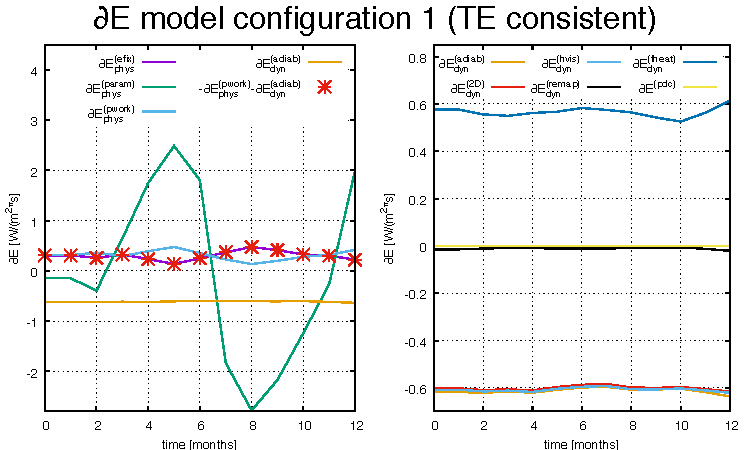
\includegraphics[width=35pc]{figs/dEdt.pdf}
 \caption{{\color{red}{[in note form] Note that the parameterizations have a closed energy budget so the fluctuations in the energy change due to parameterizations is balanced by fluxes in/out of the physics columns. The purpose of this Figure is to show that the energy tendency in the dynamical core is quite constant (to within ~0.2 $W/m^2$ or less); so only one month simulation may be enough to assess energy diagnostics for the dynamical core. DME adjust fluctuates with the physics forcing; obviously the energy fixers fluctuates with DME adjust. The {\em{consistency check}} (triangles) shows that the energy fixer exactly compensates for TE loss in dynamical core and dme adjust (there are no physics dynamics coupling errors in this configuration).}}based on monthly mean values!!}
 \label{fig:dEdt(t)}
  \end{figure}




\subsection{TE consistent configuration: state-update physics-dynamics coupling ($ftype=1$) and no TE formula discrepancy}
This configuration is the most energetically consistent in that the physical parameterizations and the continuous equations of motion on which the dynamical is based, conserve the same TE (defined in equation \eqref{eq:Ephys}); and there are no spurious sources/sinks in physics-dynamics coupling. Energetic consistency in dynamics and physics is obtained by setting $c_p^{(\ell)}\equiv c_p^{d}$ and $\mathcal{L}_{all}=\left\{ `d`,`wv`\right\}$ in the dynamical core equations of motion and TE computations. Namelist changes resulting in this configuration are $\tt{lcp\_moist}=.true.$, $\tt{se\_qsize\_condensate\_loading=1}$, and $\tt{ftype=1}$.
%If the parameterizations effectively update the model state then there are no physics-dynamics coupling errors \citep[$\tt{ftype=1}$ setup described in detail in ][]{LetAl2018JAMES}. 

The TE consistent configuration in AMIP-type simulation ({\em{F2000climo}}) is used to compute baseline TE tendencies which will be used to compute/compare with other model configurations/setups. First it is established how long an average is needed to get robust TE tendency estimates. Figure \ref{fig:dEdt(t)} shows $\partial \gi{E}$ for various aspects of CAM-SE as a function of time. First lets focus on the left plot. The TE tendency from parameterizations ($\partial \gi{E}^{(param)}_{phys}$) show significant variability with an amplitude of approximately 2.5$W/(m^2s)$. As noted above this term does not figure in the spurious TE budget. That said, the variability is reflected on to the TE tendency due to pressure work $\partial \gi{E}^{(pwork)}_{phys}\approx 0.31\pm 0.08 W/(m^2s)$. On the scale used in the left-hand plot the TE tendency of the adiabatic dynamical core $\partial \gi{E}^{(adiab)}_{dyn}$ does not seem to be affected by $\partial \gi{E}^{(param)}_{phys}$ or $\partial \gi{E}^{(pwork)}_{phys}$ in terms of variability, and remains stable at approximately 0.6$W/(m^2s)\pm ~0.02 W/(m^2s)$. The TE fixer, in this model configuration, fixes $\partial \gi{E}^{(adiab)}_{dyn}$ and $\partial \gi{E}^{(pwork)}_{phys}$. Since the TE in the adiabatic dynamics remains approximately constant and the TE tendency associated with pressure work has variability, the TE tendency from the $\partial \gi{E}^{(efix)}_{phys}$ has variability; $\partial \gi{E}^{(efix)}_{phys}\approx 0.30 \pm 0.08 W/(m^2s)$. As a consistency check $-\partial \gi{E}^{(adiab)}_{dyn}-\partial \gi{E}^{(pwork)}_{phys}$ is plotted with asterisk's and they coincide (as expected) with $\partial \gi{E}^{(efix)}_{phys}$.

The right-hand plot in  Figure \ref{fig:dEdt(t)} shows a breakdown of the dynamical core TE tendencies. The majority of the TE dissipation is due to hyperviscosity on temperature and pressure, $\partial \gi{E}^{(hvis)}_{dyn}\approx -0.61\pm 0.01 W/(m^2s)$. The diffusion of momentum is added back as frictional heating and is therefore not part of $\partial \gi{E}^{(hvis)}_{dyn}$. The frictional heating is a significant term in the TE tendency budget $\partial \gi{E}^{(fheat)}_{dyn}\approx 0.56\pm 0.02 W/(m^2s)$ and exhibits some variability but with a rather small amplitude. The remaining TE dissipation in the floating Lagrangian dynamics is inviscid dissipation and time-truncation errors $\partial \gi{E}_{dyn}^{(res)}=\partial \gi{E}_{dyn}^{({2D})}-\partial \gi{E}_{dyn}^{({hvis})}\approx 0.007 W/(m^2s)$. The TE tendency from vertical remapping is approximately $\partial \gi{E}_{dyn}^{({remap})}\approx -0.01 W/(m^2s)$. To within $~0.02 W/(m^2s)$ the dynamical core TE tendency terms can be computed from just one months average. The TE tendencies computed in physics exhibit more variability and are only accurate to $~0.1 W/(m^2s)$ after a one month average (excluding $\partial \gi{E}^{(param)}_{phys}$). 

{\color{red}{$\partial \gi{E}^{(pdc)}$ computed with \eqref{eq:pdc} is $3.709e-09$ and $\partial \gi{E}^{(pdc)}$ computed with \eqref{eq:pdc3} is $1.265e-05$. Why this discrepency? Can we consider this noise!}} 

While it is advantageous to use $ftype=1$ (state-update) physics-dynamics coupling algorithm in terms if having no spurious TE tendency from coupling ($\partial \gi{E}^{({pdc})}=0$), it does results in spurious gravity waves in the simulations. For example, Figure \ref{fig:abs_dpsdt}a shows a 1 year average of $|\frac{dp_s}{dt}|$ and it clearly exhibits unphysical oscillations coinciding with element boundaries. Details of the spectral-element method, its coupling to physics and associated noise issues are discussed in detail in \citet{HetAl2018MWR}. The gravity wave noise in the solutions are even visible in the 500hPa pressure velocity annual average (Figure \ref{fig:omega500}a). This issue can be alleviated by using a shorter physics time-step so that the physics increments are smaller (not shown). Climate modelers have historically not pursued a shorter physics time-step in production configurations as climate parameterizations are computationally expensive and there is a large sensitivity to physics time-steps in the simulated climate \citep[e.g.][]{WO2003QJR,WetAl2015JAMES}.

\subsection{Non-TE conservative ('dribbling') physics-dynamics coupling ($ftype=0,2$)}\label{se:pdc_problem}
\subsubsection{Element boundary noise}
When switching to $ftype=0$ physics-dynamics coupling algorithm in which the tendencies from physics are added throughout the dynamics (in this case twice per physics time-step) then the noise issue disappears (Figure \ref{fig:abs_dpsdt}b and \ref{fig:omega500}b). That said, there are issues with this approach. One being that the tracer mass budgets may be violated. This is illustrated in Figure \ref{fig:ftype_schematic} as explained in the next paragraph. 

The orange curve on Figure \ref{fig:ftype_schematic}a, b, d, and e is the initial state of, e.g., cloud liquid mixing ratio as a function of location, e.g., longitude. Cloud liquid is zero outside of clouds and hence a good example for the purpose of this illustration. The light blue errors show the increments (in terms of length of arrow) computed by the parameterizations based on the initial state. With $ftype=1$ the increments from physics are added to the dynamical core state (dotted line on \ref{fig:ftype_schematic}b)) before the dynamical core advances the solution in time. The parameterizations are designed to not drive the mixing ratios negative. Then the dynamical core advects the distribution (solid curve on Figure \ref{fig:ftype_schematic}c). With $ftype=0$ the physics increments are split into equal chunks (in this illustration two; blue errors on Figure \ref{fig:ftype_schematic}d). Half of the physics increments are added to the initial state (dotted line on Figure \ref{fig:ftype_schematic}e) and then dynamics advects the distribution half of the total dynamical core steps (dashed line on Figure \ref{fig:ftype_schematic}e). Then the other half of the physics increments are applied (in the same location as they were computed by physics). Now after the advection step the distribution has moved and the mixing ratio may be zero (or less than the increment) where the physics forcing is applied (e.g., left side of dashed curve). Hence the physics increment is driving the mixing ratios negative in those locations. Thereafter the distribution is advected (solid curve on Figure \ref{fig:ftype_schematic}f). In CAM the increments added in the dynamical core are limited so that they drive the mixing to zero (and not negative) if this problem occurs. This leads to a net source of mass compared to what the parameterizations prescribe (see Figure \ref{fig:pdc}). This issue also been discussed in \cite{water-leak} in the context of sea-level rise.

The majority of the noise with $ftype=1$ physics-dynamics coupling method comes from momentum sources/sinks and heating/cooling. A way alleviate noise problems and, at the same time, close the tracer mass budgets (in physics-dynamics coupling) is to use $ftype=1$ coupling for tracers and $ftype=0$ coupling for momentum and temperature. Figure \ref{fig:abs_dpsdt}c shows the noise diagnostic $|\frac{dp_s}{dt}|$ for $ftype=2$ coupling where momentum and temperature coupling uses $ftype=0$ (`dribbling') and tracers use mass-conservative $ftype=1$ coupling. Figure \ref{fig:abs_dpsdt}c looks very similar to Figure \ref{fig:abs_dpsdt}b but there is some noise near element boundaries. That said, in terms of vertical pressure velocities $ftype=2$ and $ftype=0$ climates are similar in terms of level of noise (Figure \ref{fig:omega500}b and c). The element noise in CAM-SE with $ftype=2$ seen in both $|\frac{dp_s}{dt}|$ and 500hPa pressure velocity can be `removed' by using CAM-SE-CSLAM (Figure \ref{fig:abs_dpsdt}d) which uses a quasi equal-area physics grid and CSLAM \cite[Conservative Semi-LAgrangian Multi-tracer; ][]{LNU2010JCP} consistently coupled to the SE method \citep{LTOUNGK2017MWR,HetAl2018MWR}. The noise patterns in vertical velocity of the coast off the western coast of South America are present in all CAM-SE simulations (and hence not related to physics-dynamics coupling algorithm) are also `removed' by using CAM-SE-CSLAM.
\subsubsection{Spurious TE tendencies from physics-dynamics coupling}
When using the same TE formula in the dynamical core and physics the spurious TE tendency from physics-dynamics coupling can be assessed. Since the pressure fields evolve during `dribbling' of physics forcing the TE increments from the forcing change. For $ftype=0$ and $ftype=2$ this tendency is $\partial \gi{E}^{({pdc})}=-0.05 W/(m^2s)$ and thus rather small compared to the viscosity TE dissipation rates. Since $\partial \gi{E}^{({pdc})}$ are the same (to the second digit) for $ftype=0$ and $ftype=2$ it is the momentum and temperature `dribbling' errors that dominate $\partial \gi{E}^{({pdc})}$.
\subsection{TE formula discrepancy errors}
To assess the error due to a discrepancy in the energy formula used in dynamics and physics a simulation using $ftype=1$ (no `dribbling' errors) and thermodynamically active condensate in the dynamical core ($qsize\_condensate\_loading=5$). Despite the dynamical core now using a more comprehensive formula for energy, the TE dissipation terms in the dynamical core are roughly the same as in the energy consistent versions of the model. Using \eqref{eq:discre} we can assess the TE energy discrepancy errors, $~0.59W/m^2s$. The continuous equations of motion in the dynamical core conserve an energy different from physics, and the energy fixer will restore the `physics' version of energy. This inconsistency is due to the evolutionary nature of CAM development and it is the intention to remove this inconsistency in future versions of the model.
\subsection{Limiters on vertical remapping of momentum}
CAM-SE uses a floating Lagrangian vertical coordinate \citep{S1945JAS,L2004MWR} which requires the remapping of the atmospheric state from floating levels back to reference levels. The mapping algorithms is based on the scalar conserative PPM (Piecewise Parabolic Method) with options for shape-preserving limiters. In CAM-SE momentum components and internal energy are used as the variables mapped in the vertical \citep{LetAl2018JAMES} and, contrary to earlier versions of CAM-SE, there is no limiter on the remapping of wind components. If the shape-preserving limieter is used then the TE dissipation increases by over an order of magnitude from $~0.01W/m^2s$ to $~0.2W/m^ss$. 
\subsection{Simplified surface: QPC6}
When running the model in Aqua-planet mode one can assess the effect simplifying the surface boundary condition. In particular, without topography forcing the dynamical core is not challenges with respect to stationary near-grid-scale forcing. The TE tendency with respect to pressure work remains the same $\partial \gi{E}_{phys}^{({pwork})}$ as the AMIP-tpe simulations, however, the adiabatic dynamical core TE tendency resudes to $\partial \gi{E}_{dyn}^{({adiab})}=-0.14 W/(M^2s)$. Most of that reduction is due to viscosity $\partial \gi{E}_{dyn}^{(hvis)}=-0.13 W/(M^2s)$. The frictional heating is roughtly the same as AMIP $\partial \gi{E}_{dyn}^{(fheat)}=0.48 W/(m^2s)$ as is the vertical remapping  $\partial \gi{E}_{dyn}^{(remap)}=-0.01 W/(m^2s)$. To evaluate the dynamical cores diffusion of TE it is therefore important to asses the model in a configuration with topopgrahy as the wave dynamics generated topography leads to more active diffusion operators.
\subsection{Simplified physics (no moisture): FHS94}
Simplifying the setup even further by replacing the parameterizations with relaxation towards a zonally symmetric temeprature profile and simple boundary layer friction (Held-Suarez forcing) as well as no moisture, the TE diffusion in the dynamical core decreases furhter tp $~0.002W/m^ss$. Hyperviscosity is less active leading to significant reductions compared to Aqua-planet and `real-world' simulation results. The TE diffusion in vertical remapping reduces by an order of magnitude compared to the Aqua-planet simulations ($~0.0005W/m^2s$). This further emphasizes that TE diffusion assessment in a simplified setup is not necessarily telling for the dynamical cores performance with moist physics and topography.

 \begin{figure}[h]
 \centering
 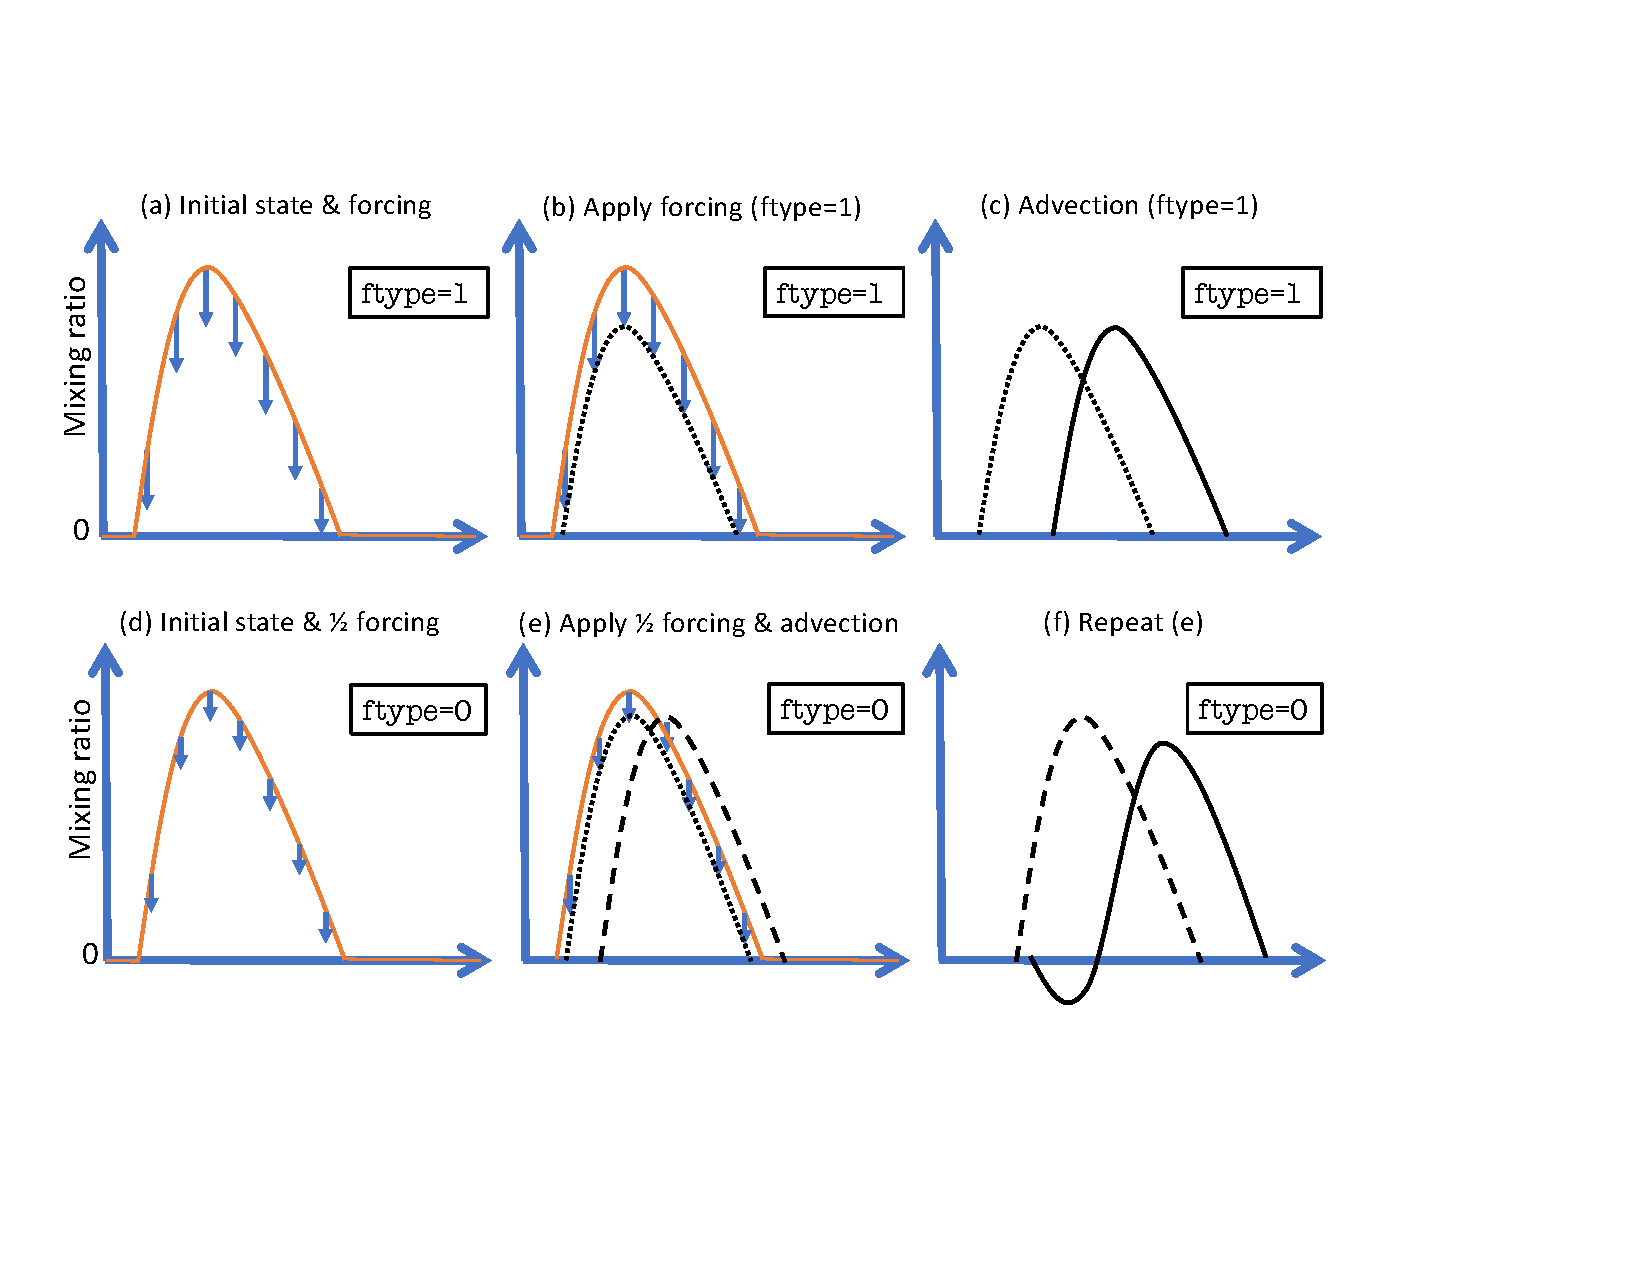
\includegraphics[width=35pc]{figs/ftype_schematic.pdf}
 \caption{A schematic of state-update ($ftype=1$; row 1) and `dribbling' ($ftype=0$; row 2) physics-dynamics coupling algorithms. See Section \ref{se:pdc_problem} for details.}
 \label{fig:ftype_schematic}
  \end{figure}

\subsection{Configuration 3: CMIP6 version}
`The discrepancy between the more comprehensive energy formula \eqref{eq:comprehensice_energy} and the CAM physics formula for TE is about 0.5 $W/m^2$ \citep{T2011LNCSEb}. By only including dry air and water vapor   in $\rho$ and setting $c_p^{(wv)}= c_p^{(d)}$ in the equations of motion, the dynamical core (in the absence of truncation errors) will conserve the energy used in CAM physics.'


 \begin{sidewaysfigure}
 \centering
 \includegraphics[width=55pc]{figs/abs_dpsdt.pdf}
 \caption{}
 \label{fig:abs_dpsdt}
  \end{sidewaysfigure}


 \begin{sidewaysfigure}
 \centering
 \includegraphics[width=55pc]{figs/omega500.pdf}
 \caption{Same as Figure \ref{fig:abs_dpsdt} but for 500hPa vertical pressure velocity.}
 \label{fig:omega500}
  \end{sidewaysfigure}

 \begin{sidewaysfigure}
 \centering
 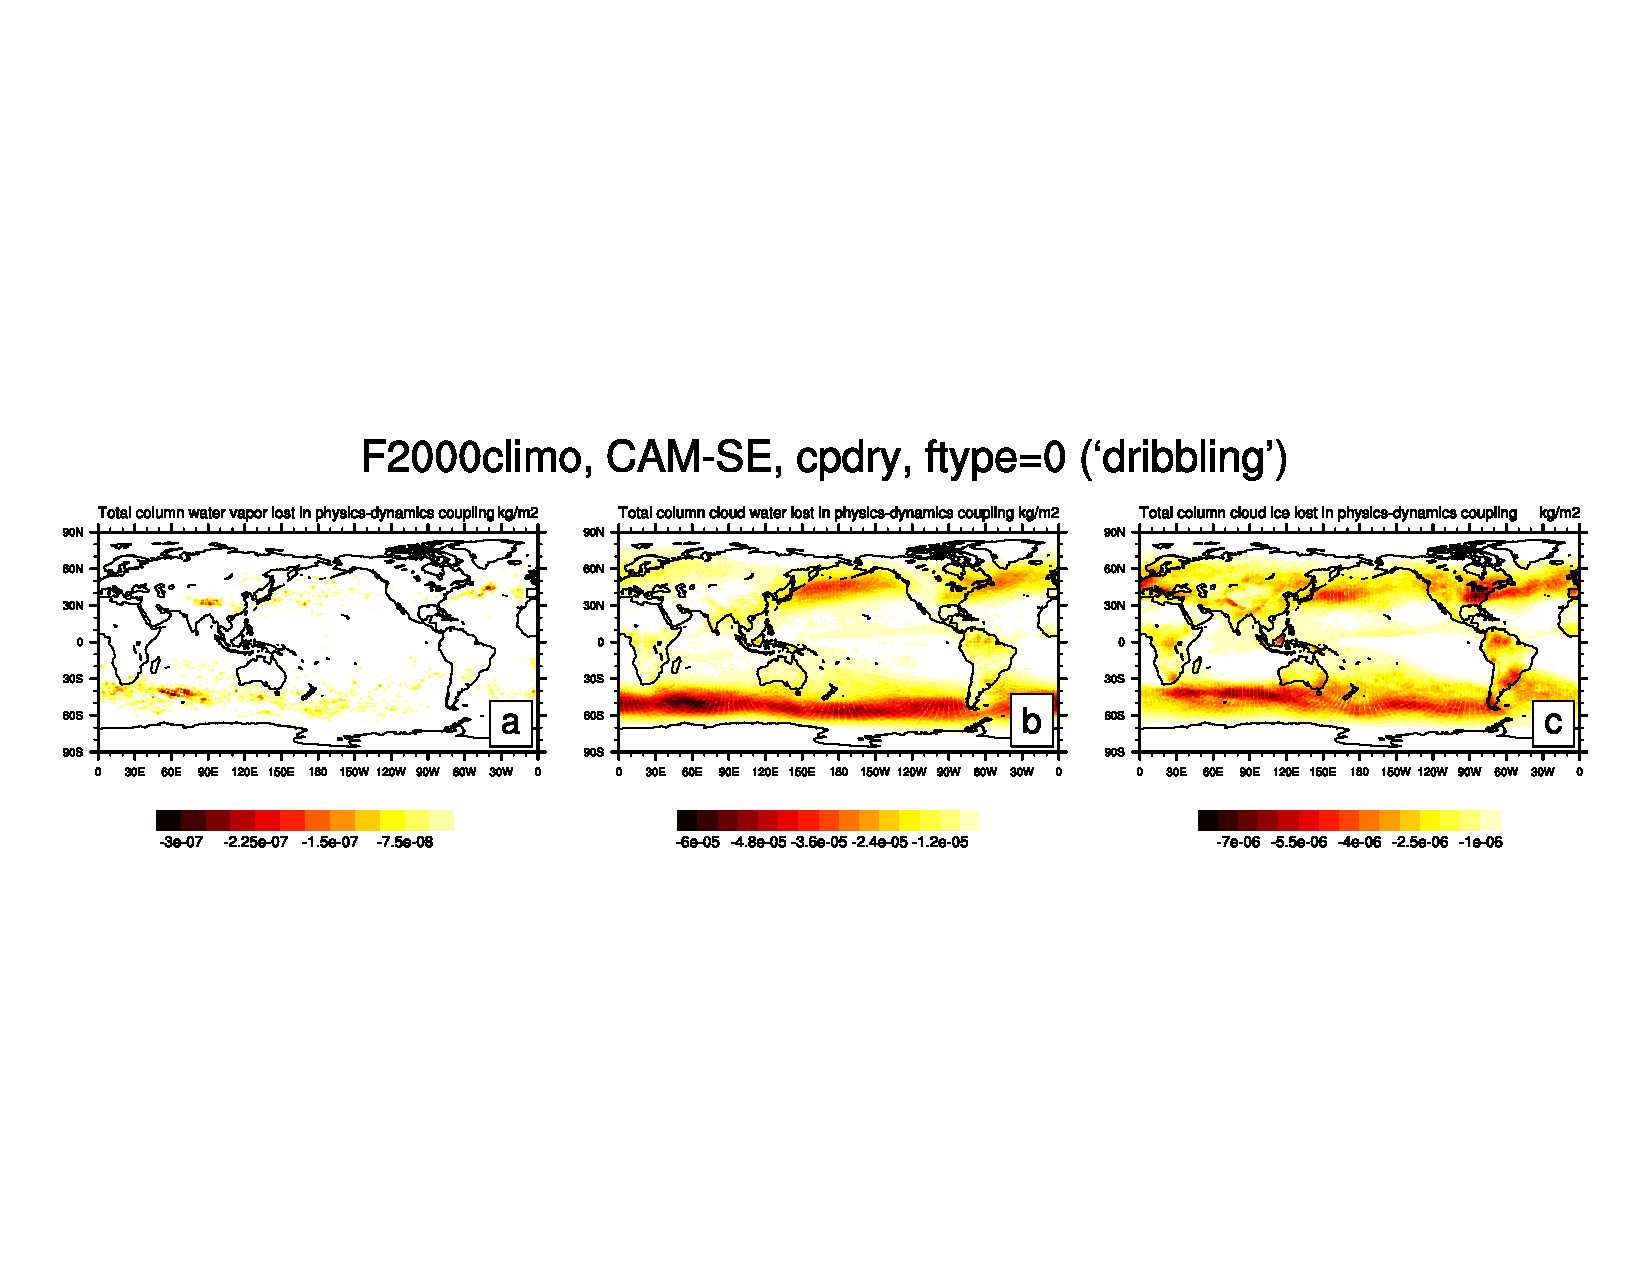
\includegraphics[width=55pc]{figs/pdc.pdf}
 \caption{Mass per unit area `clipped' in physics-dynamics coupling (so that state is not driven negative) when using $ftype=0$ (`dribbling') for (a) water vapor, (b) cloud liquid and (c) cloud ice, respectively. Interestingly the element boundaries systematically show in the plots which is likely related to the anisotropy of the quadrature grid \citep{HetAl2018MWR}.}
 \label{fig:pdc}
  \end{sidewaysfigure}


\section{Conclusions}\label{sec:concl}

%Text here ===>>>

%%
%  Numbered lines in equations:
%  To add line numbers to lines in equations,
%  \begin{linenomath*}
%  \begin{equation}
%  \end{equation}
%  \end{linenomath*}



%% Enter Figures and Tables near as possible to where they are first mentioned:
%
% DO NOT USE \psfrag or \subfigure commands.
%
% Figure captions go below the figure.
% Table titles go above tables;  other caption information
%  should be placed in last line of the table, using
% \multicolumn2l{$^a$ This is a table note.}
%
%----------------
% EXAMPLE FIGURE
%
% \begin{figure}[h]
% \centering
% when using pdflatex, use pdf file:
% \includegraphics[width=20pc]{figsamp.pdf}
%
% when using dvips, use .eps file:
% \includegraphics[width=20pc]{figsamp.eps}
%
% \caption{Short caption}
% \label{figone}
%  \end{figure}
%
% ---------------
% EXAMPLE TABLE
%
% \begin{table}
% \caption{Time of the Transition Between Phase 1 and Phase 2$^{a}$}
% \centering
% \begin{tabular}{l c}
% \hline
%  Run  & Time (min)  \\
% \hline
%   $l1$  & 260   \\
%   $l2$  & 300   \\
%   $l3$  & 340   \\
%   $h1$  & 270   \\
%   $h2$  & 250   \\
%   $h3$  & 380   \\
%   $r1$  & 370   \\
%   $r2$  & 390   \\
% \hline
% \multicolumn{2}{l}{$^{a}$Footnote text here.}
% \end{tabular}
% \end{table}

%% SIDEWAYS FIGURE and TABLE 
% AGU prefers the use of {sidewaystable} over {landscapetable} as it causes fewer problems.
%
% \begin{sidewaysfigure}
% \includegraphics[width=20pc]{figsamp}
% \caption{caption here}
% \label{newfig}
% \end{sidewaysfigure}
% 
%  \begin{sidewaystable}
%  \caption{Caption here}
% \label{tab:signif_gap_clos}
%  \begin{tabular}{ccc}
% one&two&three\\
% four&five&six
%  \end{tabular}
%  \end{sidewaystable}

%% If using numbered lines, please surround equations with \begin{linenomath*}...\end{linenomath*}
%\begin{linenomath*}
%\begin{equation}
%y|{f} \sim g(m, \sigma),
%\end{equation}
%\end{linenomath*}

%%% End of body of article

%%%%%%%%%%%%%%%%%%%%%%%%%%%%%%%%
%% Optional Appendix goes here
%
% The \appendix command resets counters and redefines section heads
%
% After typing \appendix
%
%\section{Here Is Appendix Title}
% will show
% A: Here Is Appendix Title
%
\appendix
   \section{...}

%\section{Here is a sample appendix}

%%%%%%%%%%%%%%%%%%%%%%%%%%%%%%%%%%%%%%%%%%%%%%%%%%%%%%%%%%%%%%%%
%
% Optional Glossary, Notation or Acronym section goes here:
%
%%%%%%%%%%%%%%  
% Glossary is only allowed in Reviews of Geophysics
%  \begin{glossary}
%  \term{Term}
%   Term Definition here
%  \term{Term}
%   Term Definition here
%  \term{Term}
%   Term Definition here
%  \end{glossary}

%
%%%%%%%%%%%%%%
% Acronyms
%   \begin{acronyms}
%   \acro{Acronym}
%   Definition here
%   \acro{EMOS}
%   Ensemble model output statistics 
%   \acro{ECMWF}
%   Centre for Medium-Range Weather Forecasts
%   \end{acronyms}

%
%%%%%%%%%%%%%%
% Notation 
%   \begin{notation}
%   \notation{$a+b$} Notation Definition here
%   \notation{$e=mc^2$} 
%   Equation in German-born physicist Albert Einstein's theory of special
%  relativity that showed that the increased relativistic mass ($m$) of a
%  body comes from the energy of motion of the body—that is, its kinetic
%  energy ($E$)—divided by the speed of light squared ($c^2$).
%   \end{notation}




%%%%%%%%%%%%%%%%%%%%%%%%%%%%%%%%%%%%%%%%%%%%%%%%%%%%%%%%%%%%%%%%
%
%  ACKNOWLEDGMENTS
%
% The acknowledgments must list:
%
% •	All funding sources related to this work from all authors
%
% •	Any real or perceived financial conflicts of interests for any
%	author
%
% •	Other affiliations for any author that may be perceived as
% 	having a conflict of interest with respect to the results of this
% 	paper.
%
% •	A statement that indicates to the reader where the data
% 	supporting the conclusions can be obtained (for example, in the
% 	references, tables, supporting information, and other databases).
%
% It is also the appropriate place to thank colleagues and other contributors. 
% AGU does not normally allow dedications.


\acknowledgments
The National Center for Atmospheric Research is sponsored by the National Science Foundation. We thank NCAR's Computational and Information Systems Laboratory (CISL) and NCAR's Climate and Global Dynamics division (CGD) for computational resources.

%We thank two anonymous reviewers for their helpful comments and time put into reviewing this very long/technical paper. Herrington, Reed and Lauritzen are grateful to the NCAR Advance Study Program graduate visitor program for funding Herrington's 9-month visit to NCAR. We thank NCAR's Computational and Information Systems Lab (CISL) for providing computing support. Goldhaber was partially supported by the U.S. Department of Energy Office of Biological and Environmental Research, Work Package 12-015334 ``Multiscale Methods for Accurate, Efficient, and Scale-Aware Models of the Earth System''. Medeiros acknowledges support by the Regional and Global Climate Modeling Program of the U.S. Department of Energy's Office of Science,  Cooperative Agreement DE-FC02-97ER62402. Benedict was funded by National Science Foundation (NSF) Rapid Response Research (RAPID) award AGS-1547910. The data presented in this manuscript is available at {\url{https://github.com/PeterHjortLauritzen/2017-JAMES-CESM2-SE.git}}.

%% ------------------------------------------------------------------------ %%
%% Citations

% Please use ONLY \citet and \citep for reference citations.
% DO NOT use other cite commands (e.g., \cite, \citeyear, \nocite, \citealp, etc.).


%% Example \citet and \citep:
%  ...as shown by \citet{Boug10}, \citet{Buiz07}, \citet{Fra10},
%  \citet{Ghel00}, and \citet{Leit74}. 

%  ...as shown by \citep{Boug10}, \citep{Buiz07}, \citep{Fra10},
%  \citep{Ghel00, Leit74}. 

%  ...has been shown \citep [e.g.,][]{Boug10,Buiz07,Fra10}.



%%  REFERENCE LIST AND TEXT CITATIONS

\bibliography{bib}
%
% Either type in your references using
%
% \begin{thebibliography}{}
% \bibitem[{\textit{Kobayashi et~al.}}(2003)]{R2013} Kobayashi, T.,
% Tran, A.~H., Nishijo, H., Ono, T., and Matsumoto, G.  (2003).
% Contribution of hippocampal place cell activity to learning and
% formation of goal-directed navigation in rats. \textit{Neuroscience}
% 117, 1025--1035.
%
% \bibitem{}
% Text
% \end{thebibliography}
%
%\bibliography{bib}
%%%%%%%%%%%%%%%%%%%%%%%%%%%%%%%%%%%%%%%%%%%%%%%
% Or, to use BibTeX:
%
% Follow these steps
%
% 1. Type in \bibliography{<name of your .bib file>} 
%    Run LaTeX on your LaTeX file.
%
% 2. Run BiBTeX on your LaTeX file.
%
% 3. Open the new .bbl file containing the reference list and
%   copy all the contents into your LaTeX file here.
%
% 4. Run LaTeX on your new file which will produce the citations.
%
% AGU does not want a .bib or a .bbl file. Please copy in the contents of your .bbl file here.


%% After you run BibTeX, Copy in the contents of the .bbl file here:


%%%%%%%%%%%%%%%%%%%%%%%%%%%%%%%%%%%%%%%%%%%%%%%%%%%%%%%%%%%%%%%%%%%%%
% Track Changes:
% To add words, \added{<word added>}
% To delete words, \deleted{<word deleted>}
% To replace words, \replace{<word to be replaced>}{<replacement word>}
% To explain why change was made: \explain{<explanation>} This will put
% a comment into the right margin.

%%%%%%%%%%%%%%%%%%%%%%%%%%%%%%%%%%%%%%%%%%%%%%%%%%%%%%%%%%%%%%%%%%%%%
% At the end of the document, use \listofchanges, which will list the
% changes and the page and line number where the change was made.

% When final version, \listofchanges will not produce anything,
% \added{<word or words>} word will be printed, \deleted{<word or words} will take away the word,
% \replaced{<delete this word>}{<replace with this word>} will print only the replacement word.
%  In the final version, \explain will not print anything.
%%%%%%%%%%%%%%%%%%%%%%%%%%%%%%%%%%%%%%%%%%%%%%%%%%%%%%%%%%%%%%%%%%%%%

%%%
\listofchanges
%%%

\end{document}

%%%%%%%%%%%%%%%%%%%%%%%%%%%%%%%%%%%%%
%% Supporting Information
%% (Optional) See AGUSuppInfoSamp.tex/pdf for requirements 
%% for Supporting Information.
%%%%%%%%%%%%%%%%%%%%%%%%%%%%%%%%%%%%%



%%%%%%%%%%%%%%%%%%%%%%%%%%%%%%%%%%%%%%%%%%%%%%%%%%%%%%%%%%%%%%%

More Information and Advice:

%% ------------------------------------------------------------------------ %%
%
%  SECTION HEADS
%
%% ------------------------------------------------------------------------ %%

% Capitalize the first letter of each word (except for
% prepositions, conjunctions, and articles that are
% three or fewer letters).

% AGU follows standard outline style; therefore, there cannot be a section 1 without
% a section 2, or a section 2.3.1 without a section 2.3.2.
% Please make sure your section numbers are balanced.
% ---------------
% Level 1 head
%
% Use the \section{} command to identify level 1 heads;
% type the appropriate head wording between the curly
% brackets, as shown below.
%
%An example:
%\section{Level 1 Head: Introduction}
%
% ---------------
% Level 2 head
%
% Use the \subsection{} command to identify level 2 heads.
%An example:
%\subsection{Level 2 Head}
%
% ---------------
% Level 3 head
%
% Use the \subsubsection{} command to identify level 3 heads
%An example:
%\subsubsection{Level 3 Head}
%
%---------------
% Level 4 head
%
% Use the \subsubsubsection{} command to identify level 3 heads
% An example:
%\subsubsubsection{Level 4 Head} An example.
%
%% ------------------------------------------------------------------------ %%
%
%  IN-TEXT LISTS
%
%% ------------------------------------------------------------------------ %%
%
% Do not use bulleted lists; enumerated lists are okay.
% \begin{enumerate}
% \item
% \item
% \item
% \end{enumerate}
%
%% ------------------------------------------------------------------------ %%
%
%  EQUATIONS
%
%% ------------------------------------------------------------------------ %%

% Single-line equations are centered.
% Equation arrays will appear left-aligned.

Math coded inside display math mode \[ ...\]
 will not be numbered, e.g.,:
 \[ x^2=y^2 + z^2\]

 Math coded inside \begin{equation} and \end{equation} will
 be automatically numbered, e.g.,:
 \begin{equation}
 x^2=y^2 + z^2
 \end{equation}


% To create multiline equations, use the
% \begin{eqnarray} and \end{eqnarray} environment
% as demonstrated below.
\begin{eqnarray}
  x_{1} & = & (x - x_{0}) \cos \Theta \nonumber \\
        && + (y - y_{0}) \sin \Theta  \nonumber \\
  y_{1} & = & -(x - x_{0}) \sin \Theta \nonumber \\
        && + (y - y_{0}) \cos \Theta.
\end{eqnarray}

%If you don't want an equation number, use the star form:
%\begin{eqnarray*}...\end{eqnarray*}

% Break each line at a sign of operation
% (+, -, etc.) if possible, with the sign of operation
% on the new line.

% Indent second and subsequent lines to align with
% the first character following the equal sign on the
% first line.

% Use an \hspace{} command to insert horizontal space
% into your equation if necessary. Place an appropriate
% unit of measure between the curly braces, e.g.
% \hspace{1in}; you may have to experiment to achieve
% the correct amount of space.


%% ------------------------------------------------------------------------ %%
%
%  EQUATION NUMBERING: COUNTER
%
%% ------------------------------------------------------------------------ %%

% You may change equation numbering by resetting
% the equation counter or by explicitly numbering
% an equation.

% To explicitly number an equation, type \eqnum{}
% (with the desired number between the brackets)
% after the \begin{equation} or \begin{eqnarray}
% command.  The \eqnum{} command will affect only
% the equation it appears with; LaTeX will number
% any equations appearing later in the manuscript
% according to the equation counter.
%

% If you have a multiline equation that needs only
% one equation number, use a \nonumber command in
% front of the double backslashes (\\) as shown in
% the multiline equation above.

% If you are using line numbers, remember to surround
% equations with \begin{linenomath*}...\end{linenomath*}

%  To add line numbers to lines in equations:
%  \begin{linenomath*}
%  \begin{equation}
%  \end{equation}
%  \end{linenomath*}



%Descriptor & $\mathcal{N}$ & $c_p^{(\ell)}$ &  $ftype$ & $\partial \gi{E}_{phys}^{({param})}$ & $\partial \gi{E}_{phys}^{({pwork})}$ &  $\partial \gi{E}_{phys}^{({efix})}$ &  $\partial \gi{E}_{phys}^{({discr})}$ &  $\partial \gi{E}_{dyn}^{({2D})}$ & $\partial \gi{E}_{dyn}^{({hvis})}$ & $\partial \gi{E}_{dyn}^{({fheat})}$ & $\partial \gi{E}_{dyn}^{(res)}$ & $\partial \gi{E}_{dyn}^{(remap)}$ & $\partial \gi{E}_{dyn}^{(adiab)}$  & $\partial \gi{E}^{(pdc)}$\\
%\hline \hline \\
%consistent & 1                       & false   & 1   & -0.137&   3.12&      3& 0       &  -6.01&  -6.08&   5.65& 0.0661& -0.114&  -6.13& 2.65e-07 \\
%`dribbling' 1 & 1                       & true   & 0   &   1.02&   3.12&   3.31& 0       &  -5.93&     -6&   5.57& 0.0742& -0.106&  -6.03&  0.469\\
%`dribbling' 2 & 1                       & true   & 2   &   1.29&   3.16&   3.41& 0       &  -5.98&  -6.06&   5.63& 0.0755& -0.109&  -6.09&  0.484\\
%
%PPM limiter & 1                       & true   & 1   &   2.16&   3.17&   4.72& 0       &   -5.9&  -5.97&   5.09& 0.0648&  -1.99&  -7.89& 5.56e-08\\
%energy discr & 5                       & true   & 1   &   3.74&   3.32&  -3.13&  0.594&  -6.03&  -6.12&   5.75& 0.0915& -0.112&  -6.14&  undef\\
%FHS94       & 1                       & false  & 2  &  ?     &   0    &  -   &  0     &  -0.0248 &  -0.0248 & 0.122 &  7.79e-07 &  0.00522 &  -0.0196 & ??
